\section{はじめに}
\pagenumbering{arabic}

 従来のゲームプレイは、プレイヤーがゲームハードやゲーミングPCを所有し、その上でゲームを動作させることによって実現されている。クラウドゲーミングは、クラウドサーバ上でゲームを動作させてその画面をクライアントであるプレイヤーの端末にストリーミングすることで、ゲームをネットワーク越しにプレイすることを可能にするサービスである。プレイヤーの使用する端末は、クラウドサーバより送信されるゲーム画面の再生とプレイヤーの操作のサーバへの送信だけを行う。この仕組みによって、スマートフォンやタブレットなどの性能が貧弱なデバイスでも高価なゲームハードやゲーミングPCでプレイするのと同様の高品質なゲーム体験を得られることが期待できる。(この辺の出典どうしよう)

 商用のクラウドゲーミングサービスも展開されており、GoogleのGoogle Stadia、SONYのPlayStation NOW、NVIDIAのGeForce NOWなどがある。(もうちょっと膨らませたい気がする)

(この辺でGamingAnywhereの話とかする?)

(クラウドゲーミングは遅延が課題ですという話を論文引用しながら書く)(サーベイ論文使ったらもっといろんな課題の話できるな)
クラウドゲーミングの課題はユーザ目線で高品質な画質の担保、十分なネットワーク帯域幅の確保、伝送データ圧縮・ストリーミング技術、画面表示や操作の遅延の最小化など。プロバイダ目線でゲーム環境の仮想化、サーバにおける負荷分散

(ボランティアコンピューティングの話はBOINCの引用でいいかな)

(研究目的を書く)
クラウドのデータセンターの配置次第で著しく遅延が大きい環境でプレイするプレイヤーが存在する可能性あり。
ボランティアが提供する地理的に近傍の遊休コンピュータのリソースを利用するクラウドゲーミングフレームワークを提案。プレイヤーから見て近傍の遊休コンピュータ上でクラウドゲームサーバを動作させる。ネットワーク遅延削減によりプレイヤーが体験する遅延を減少させる

\ref{kako}節では、過去における研究について述べ、
\ref{kadai}章では、現状と今後の課題について述べる。
また、付録\ref{omake1}におまけその1を添付する。

\begin{figure*}[t]
 \centering
% 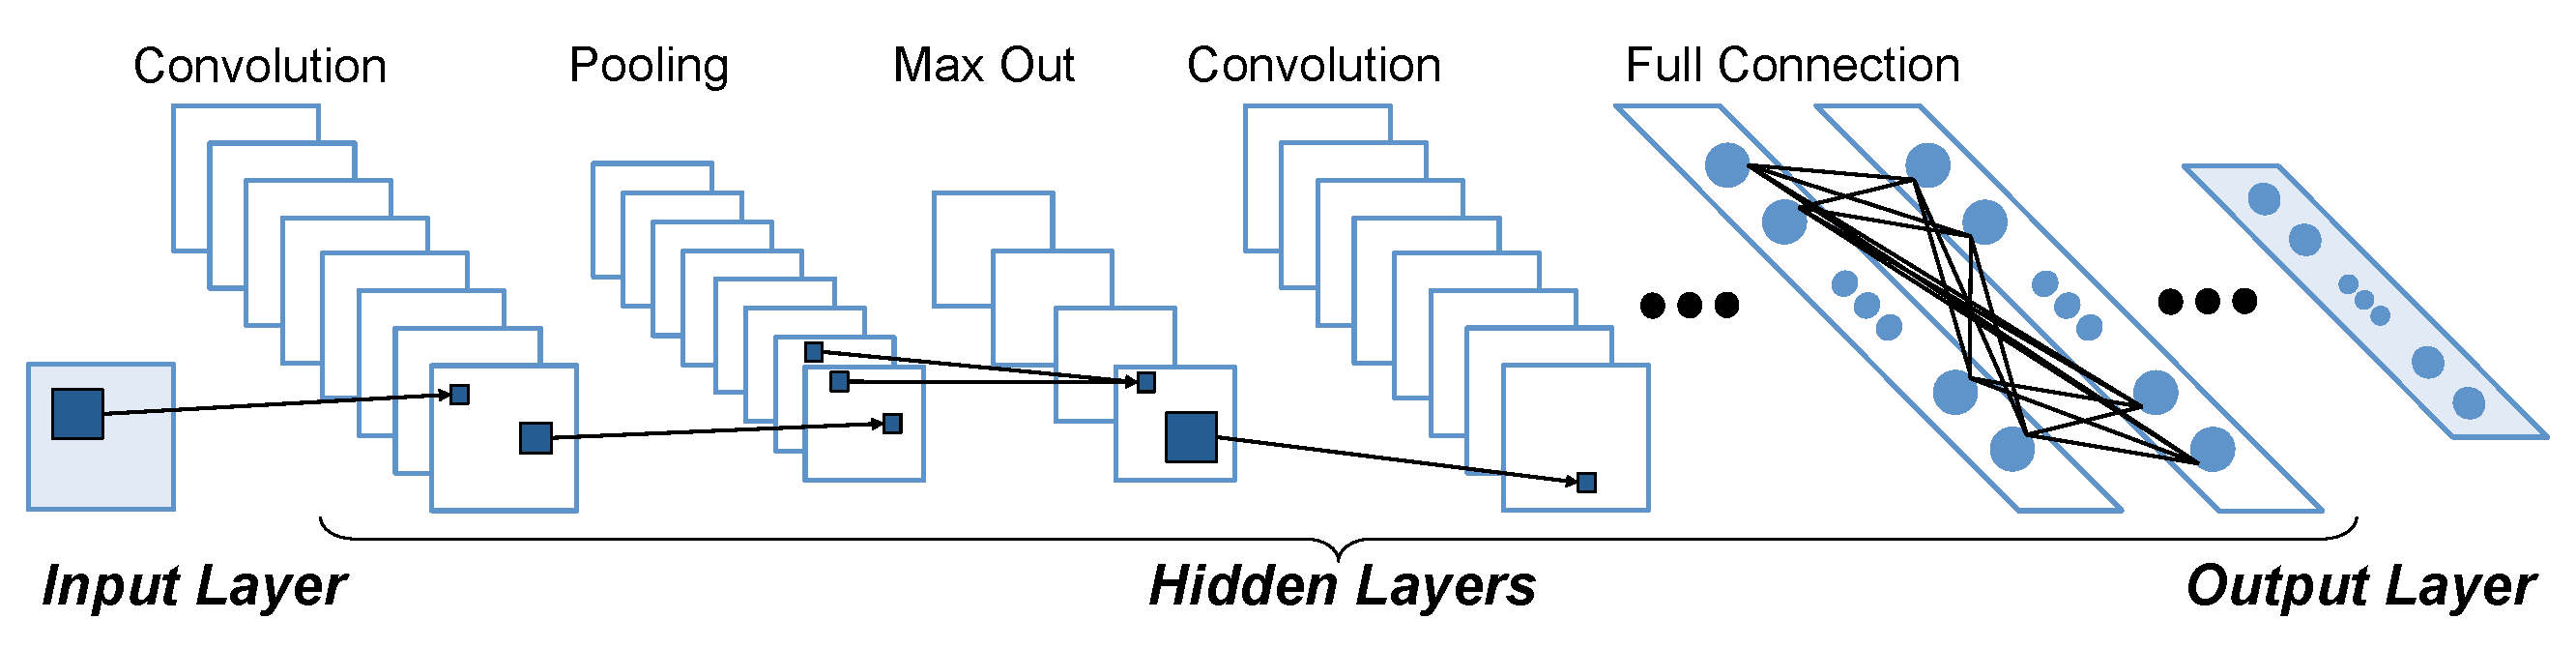
\includegraphics[width=0.8\textwidth,keepaspectratio,clip]{fig/cnn.eps}
 \caption{Convolutional Neural Network (CNN)}
 \label{fig:CNN}
\end{figure*}

過去における研究としては\cite{alex_nips12}などがある。

\begin{figure}
\centerline{ここに図を書く}
\caption{これは図の例}
\end{figure}

\begin{table}
\centerline{ここに表を書く}
\caption{これは表の例}
\end{table}


\newpage

This page is written in English. This page is written in English. 
